% !TeX root = ../main.tex

\appendix{E}{Implementation Details}\label{sec:appendix_implementation_details}


\section{Parameter Choices of DBSCAN}\label{sec:dbscan}
% (short reasons for the assignments of parameters)
% Each home location candidate can be associated with nighttime clusters containing different numbers of observed locations.
While most cases involve multiple observed locations forming a cluster around the home location candidate, it is possible that only a single observed location is associated with a home location candidate, particularly in areas with sparse base station coverage.
To account for this case, we set the \textit{min\_samples} parameter to one.
Another parameter, \textit{eps}, which defines the maximum distance for two observed locations to be considered neighbors within a cluster, is set to 5~km with distances calculated using Vincenty's formulae.
This parameter choice is motivated by the heterogeneous nature of effective service radii of base stations across our study regions.

% (connect eps to effective service redii)
Since effective service radii provide informative insights into the neighboring distances between consecutive base stations, they serve as appropriate prior knowledge for determining the \textit{eps} value.
Theoretically, neighboring distances should be less than the sum of two consecutive base stations' effective service radii.
Therefore, \textit{eps} should be greater than the maximum of all neighboring distances approximated by the sum of consecutive base stations' effective service radii but shouldn't be excessively large, as an overly large value might cause the algorithm to incorrectly merge two distinct clusters into one.
Nevertheless, we believe that individuals will stay at home most of the time, so the distance between clusters should be relatively large to mitigate the issue of misidentification of clusters.

% (explanation of the determination on our study areas' service redii)
Our study regions including Deyang, Chongqing, and other prefectures in Sichuan Province encompass diverse geographic regions, including urban, suburban, and rural areas, and typically, the service radii in urban areas is smaller than those in rural areas (\cite{zreikat2004comparative}).
\cite{zhou2024cell} provides an overview of recent research that utilizes CDRs to locate individuals' positions across various regions, including a particular discussion on spatial resolution, which is partially related to base stations' service radii.
The overview states that the average service radius in urban regions (Shanghai, Nanjing, and Guiyang) is less than 1 km, while our study regions have much more complicated compositions.
Therefore, the 5 km threshold represents an aggressive lower bound, which aims to account for the larger service radii characteristic of rural and suburban regions while maintaining meaningful spatial clustering in dense urban regions.
Besides, choosing a relatively large \textit{eps} value addresses a key trade-off: while smaller values would reduce localization accuracy in rural regions, larger values risk merging distinct urban clusters.
However, this risk can be potentially mitigated because individuals spend most time at home locations, and our weighted-average estimation across telecom stations (based on usage frequency) ensures that wrongly-included stations receive low weights in the final home estimation.


\clearpage\newpage
\section{Temporal Filtering}
\begin{algorithm}[h!]
\renewcommand{\algorithmicrequire}{\textbf{Input:}}
\renewcommand{\algorithmicensure}{\textbf{Output:}}
\caption{Home Cluster Estimation}
\label{home_cluster}
\begin{algorithmic}[1]
    \REQUIRE $C^\text{night}_i$
    \ENSURE $C^\text{home}_i$

    \STATE $\text{candidates} \leftarrow$ sort $C^\text{night}_i$ in descending order by the temporal size
    \STATE $C^\text{home}_i \leftarrow [\text{candidates}[1]]$
    \STATE

    \FORALL {$j=2,\cdots,\text{length}(\text{candidates})$}
        \STATE $\text{isolate} \gets \text{true}$
        \STATE $\text{candidate} \gets \text{candidates}[j]$
        \STATE

        \FORALL {$k=1,\cdots,\text{length}(C^\text{home}_i)$}
            \IF {$\text{candidate}$ temporally overlaps with $C^\text{home}_i[k]$}
                \STATE $\text{isolate} \gets \text{false}$
                \STATE \textbf{break}
            \ENDIF
        \ENDFOR
        \STATE

        \IF {$\text{isolate} = \text{true}$ and the temporal size of candidate $> 2$}
            \STATE insert $\text{candidate}$ into $C^\text{home}_i$
        \ENDIF
    \ENDFOR
    \STATE

    \STATE sort $C^\text{home}_i$ in ascending order by the start time of service time interval
    \STATE \textbf{return} $C^\text{home}_i$
\end{algorithmic}
\end{algorithm}

\begin{theorem}
For the algorithm \ref{home_cluster}, where each user $i \in V$ has a nighttime cluster set $C^{\text{night}}_i$ with $|C^{\text{night}}_i|$ elements, the time complexity is $O\left(\sum_{i \in V} |C^{\text{night}}_i|^2\right)$ and the space complexity is $O\left(\sum_{i \in V} |C^{\text{night}}_i|\right)$.
\end{theorem}

\begin{proof}
For the time complexity, consider the worst case scenario where for all user $i$, all nighttime clusters are temporally non-overlapping with one another. The algorithm will iterate for
$$
1+2+\ldots+(|C^{\text{night}}_i|-1) = \frac{|C^{\text{night}}_i|(|C^{\text{night}}_i|-1)}{2} = O(|C^{\text{night}}_i|^2)
$$
times for each user $i$. Aggregating over all users gives the total time complexity of $O\left(\sum_{i \in V} |C^{\text{night}}_i|^2\right)$.
For the space complexity, under the worst case scenario, the size of $C^{\text{home}}_i$ is identical to $|C^{\text{night}}_i|$ for each user $i$. Therefore, the total space required is $O\left(\sum_{i \in V} |C^{\text{night}}_i|\right)$.
\end{proof}


\section{Residential Shifts}\label{sec:migrant_criterion}
\begin{table}[htbp]
% \vspace{0.2cm}
\renewcommand{\arraystretch}{1.5}
\setlength{\tabcolsep}{4mm}{}
\centering
\small
\caption{Statistics of Migrants by the Month of Migration}
\begin{tabular}{lcccccc} \hline
& \multicolumn{3}{c}{Count of Migrants} & \multicolumn{3}{c}{Migration Distance} \\
\cline{2-4} \cline{5-7}
month & all & inter-pref. & ratio (\%) & all & inter-pref. & ratio (\%) \\ \hline
Aug. 2013 & 2434 & 2006 & 82.42 & 134.8 & 157.11 & 116.55 \\
Sep. 2013 & 974 & 797 & 81.83 & 135.82 & 159.25 & 117.25 \\
Oct. 2013 & 451 & 311 & 68.96 & 119.01 & 158.83 & 133.46 \\
Nov. 2013 & 363 & 247 & 68.04 & 101.0 & 137.35 & 135.99 \\
Dec. 2013 & 305 & 231 & 75.74 & 132.15 & 164.7 & 124.63 \\
Jan. 2014 & 448 & 338 & 75.45 & 128.04 & 160.78 & 125.57 \\
Feb. 2014 & 594 & 458 & 77.1 & 116.56 & 142.44 & 122.2 \\
Mar. 2014 & 594 & 443 & 74.58 & 118.48 & 148.91 & 125.68 \\
Apr. 2014 & 675 & 519 & 76.89 & 129.55 & 160.28 & 123.72 \\
May 2014 & 1520 & 1222 & 80.39 & 127.37 & 151.29 & 118.78 \\
\hline

\end{tabular}
\label{tab:migration_sample}%

\end{table}%

\vspace{-2em}
\begin{singlespace}
\begin{footnotesize}
\noindent Notes: The column all represents the count of migrants and migration distance are computed on the phone users who satisfy the first requirement of migrants. Therefore, they don't necessarily change their home locations to another prefecture. The column, inter-pref., means statistics are computed on the phone users who satisfy the first and second requirement of migrants. Moreover, the unit of distance is in kilometers.
\end{footnotesize}
\end{singlespace}

The treatment timing varies across users who have once changed their residential locations, but we select those who migrate in the middle of the sample period, i.e., $g \in \{4,5,6,7\}$.
For these users, we have higher confidence level to safely classify them as migrants in that the temporal sizes of the two home clusters are comparable.
For example, if the residential shift takes place in September 2013, then the first cluster's temporal size is about a month while the second cluster's temporal size is very likely to be greater than a month with a maximum of 9 months.
In this case, the two home clusters are obviously not comparable in terms of the temporal sizes, so we are less confident to classify this user as a migrant because the first cluster may be a short visit, and the first timestamp associated with the second home cluster might be even earlier, outside the sample period.
We call this kind of issue observation window bias, which results from the pre-determined observation time frame where the accumulation of information for inference is insufficient.
Referring to Table \ref{tab:migration_sample}, it seems that there are many users relocating in the early and late period of the sample period, highlighting the importance to restrict the definition of migrants to those relocate in the middle of the sample period.
Besides, restricting migrants to those who relocate in the middle of the sample period doesn't substantially distort the origin-destination distribution, as the KL-divergence is about 0.35, which is calculated by comparing the origin-destination distribution of inter-prefecture migrants who migrate in the middle of the sample period to that of migrants who migrate in all months.

We can define some parameters to rule out users who have incomparable temporal sizes of home clusters, for example, requiring the temporal sizes of the home clusters or even the ratio between them to be greater than thresholds.
Nonetheless, as aforementioned, it's not necessary to define such parameters.
We can simply follow the patterns of the data and conduct restrictive sample selection to validate the robustness of the results.
Moreover, even if these parameters are defined, they are not employed to reduce methodological error—like other existing methods to identify residential shift mentioned in Section~\ref{sec:2_residential_shift_and_internal_migration}.
Rather, it's a decision on how much we should trust the patterns

\clearpage\newpage
\begin{table}[htbp]
\vspace{0.3cm}
\renewcommand{\arraystretch}{1.6}
\setlength{\tabcolsep}{1mm}{}
\centering
\small
\caption{Balance of Pre-Treatment (Residential Shifts) Covariates}

\begin{tabular}{lcccc} \hline
Variable & Non-Migrant & Migrant & Difference & p-value \\ \hline
\textit{Panel A: Inter-Prefecture Migrants, Any} \\
age & 40.87 & 36.67 & -4.2 & 0.0 \\
male flag & 0.66 & 0.68 & 0.02 & 0.0001 \\
born in Deyang flag & 0.82 & 0.65 & -0.17 & 0.0 \\
(max) phone price & 954.72 & 1059.87 & 105.15 & 0.0 \\
(max) smartphone flag & 0.65 & 0.77 & 0.12 & 0.0 \\ \hline

\textit{Panel B: Inter-Prefecture Migrants, Middle Period} \\
age & 40.87 & 35.56 & -5.31 & 0.0 \\
male flag & 0.66 & 0.71 & 0.05 & 0.0001 \\
born in Deyang flag & 0.82 & 0.61 & -0.21 & 0.0 \\
(max) phone price & 954.72 & 1011.0 & 56.28 & 0.0234 \\
(max) smartphone flag & 0.65 & 0.74 & 0.09 & 0.0 \\ \hline

\end{tabular}
\label{tab:non_migrant_migrant_comparison}%

\end{table}%

\vspace{-3em}
\begin{singlespace}
\begin{footnotesize}
\noindent Notes: (i) Panel A presents statistics for phone users who meet the first two requirements of the migrant definition outlined in Definition \ref{def:migrants} without restricting the migration timeframe, while Panel B analyzes data based on the complete migrant definition, limiting inter-prefecture migrants to those who migrated between November 2013 and February 2014. (ii) The variables include: male flag, a binary indicator of user gender; born in Deyang flag, a binary variable indicating whether the user was born in Deyang prefecture; and (max) phone price, and (max) smartphone flag, which are time-variant variables constructed using data before November 2013 to examine pre-treatment covariates. (iii) Since phone users may have changed devices or own multiple phone devices between August 2013 and October 2013,(max) phone price represents the highest price among all phones a user owned during this period, and (max) smartphone flag indicates whether a user ever owned a smartphone during this period.
\end{footnotesize}
\end{singlespace}


% \textbf{Q: What the difference between the complete migrant sample and subsample?}

Table \ref{tab:non_migrant_migrant_comparison} presents the sample statistics of our final selection on migrants, compared to the non-migrant groups.
We can see that migrants' characteristics differ slightly between the complete migrant sample and the subsample including only those who migrate in the middle of sample period.
The differences in demographic features compared to non-migrants are larger for the subsample migrants than for the complete migrant sample, while the differences in phone-related characteristics compared to non-migrants are smaller for the subsample migrants.

% \textbf{Q: What the difference between the migrants and non-migrants?}

Examining Panel B more closely, as we define the treatment group for analysis as those who migrate across prefectures during the middle of the sample period.
Compared to non-migrants, these migrants tend to be younger and have a higher probability of being male, with a lower likelihood of being born in Deyang city.
Furthermore, they own slightly better phone devices and a higher fraction of them use smartphones.
Although the imbalance of pre-treatment covariates is significant, the scale of differences seems to be small.


\section{Smartphone Adoption}
\begin{figure}[h!]
\centering
\caption{Number of Phone Users Upgrading to Smartphones by Month}
\vspace{0.1cm}

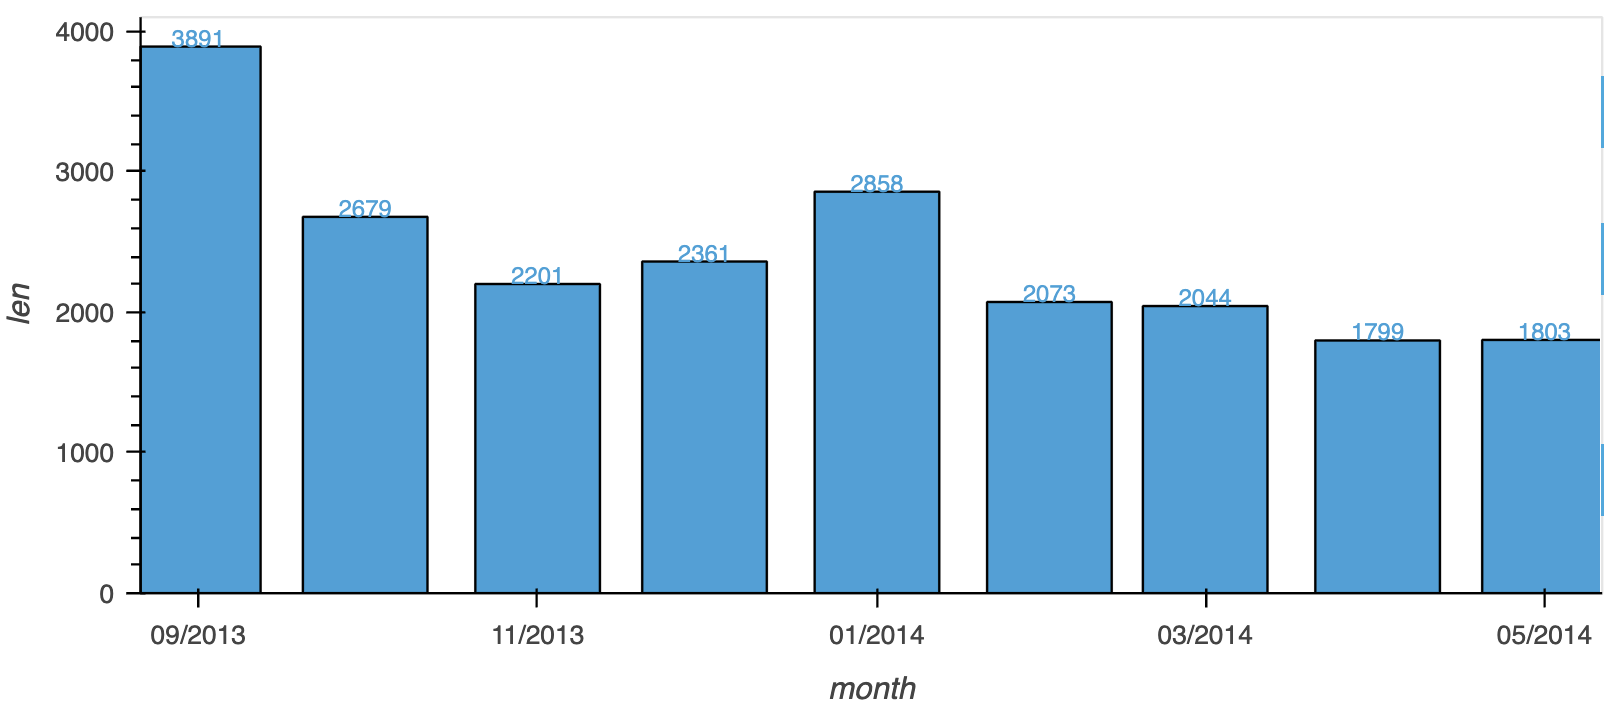
\includegraphics[scale=0.51]{figures/number_of_smartphone_adopters.png}


% \caption*{Notes: .}
\label{fig:number_of_smartphone_changers}
\end{figure}

The above figure shows the counts of smartphone adopters for each month. Generally, there are few differences across months, except a notable increase in September 2013, owing to the observation window bias.

Table~\ref{tab:non_changer_changer_comparison} shows that smartphone adopters who upgrade during middle periods are largely similar to those upgrading during any month of the sample period, with the exception of owning slightly less expensive devices.
This pattern may result from observation window bias.
Panel A includes users who switch to smartphones during early sample periods, but we lack sufficient observation periods to verify their consistent use of non-smartphone devices before adoption.


\begin{table}[htbp]
\vspace{0.5cm}
\renewcommand{\arraystretch}{1.6}
\setlength{\tabcolsep}{1.1mm}{}
\centering
\small
\caption{Balance of Pre-Treatment (Smartphone Adoption) Covariates}
\begin{tabular}{lcccc} \hline
Variable & Non-Changers & Changers & Difference & p-value \\ \hline
\textit{Panel A: Smartphone Adopters, Any} \\
age & 44.7 & 41.68 & -3.02 & 0.0 \\
male flag & 0.66 & 0.65 & 0.0 & 0.5039 \\
born in Deyang flag & 0.86 & 0.83 & -0.03 & 0.0 \\
(max) phone price & 409.9 & 706.11 & 296.22 & 0.0 \\ \hline

\textit{Panel B: Smartphone Adopters, Middle Periods} \\
age & 44.7 & 41.84 & -2.86 & 0.0 \\
male flag & 0.66 & 0.66 & 0.0 & 0.8563 \\
born in Deyang flag & 0.86 & 0.83 & -0.02 & 0.0 \\
(max) phone price & 409.9 & 501.75 & 91.85 & 0.0 \\ \hline

\end{tabular}
\label{tab:non_changer_changer_comparison}%
\end{table}%

\vspace{-2em}
\begin{singlespace}
\begin{footnotesize}
\noindent Notes: (i) The Changers refers to the smartphone adopters and non-changers mean non-smartphone users. (ii) The Panel A compares pre-treatment covariates between smartphone adopters (upgrading in any month) and non-smartphone users. Panel B examines the same comparison but restricts smartphone adopters to those upgrading between November 2013 and February 2014. (iii) The pre-treatment covariates are crafted in the same way with Table \ref{tab:non_migrant_migrant_comparison}.
\end{footnotesize}
\end{singlespace}


The definition of "changers" in Panel B of Table~\ref{tab:non_changer_changer_comparison} corresponds to our  formal definition of smartphone adopters presented in Definition~\ref{def:smartphone_adopter}.
We can see that smartphone adopters are slightly younger, marginally more likely to be born outside Deyang prefecture (by approximately 2\%), and own more expensive non-smartphone phone devices (before adoption) compared to non-smartphone users.
Besides, the age composition of the two groups shows no significant difference.
Similar to the situation in residential shifts, the imbalance seems to be not obvious.

\clearpage\newpage
\section{Selection of Anticipation Parameter}\label{sec:anticipation}
In this section, we explain how we determine the anticipation parameter $\delta$, which is the number of months allowed for anticipation.
As we aim to identify effects of residential shift and smartphone adoption on two groups of outcomes---mobility and mobile communication network features---it is plausible for migrants to change their mobility and mobile communication behavior prior to their relocations, as explained previously.
However, it's subtle whether users will anticipate upgrading their devices to smartphones.
Therefore, we will primarily focus on the residential shift as an illustration example and apply the strategy developed in this section on both treatment contexts.

To select the correct horizon of $\delta$, we initiate a warm-up estimation for the group-time ATT by applying the \cite{callaway2021difference}'s method implemented in the \textit{did} R package.\footnote{The \textit{did} R package, to which both authors of the paper, \cite{callaway2021difference}, have been contributing.}
Several critical settings include setting the \textit{anticipation} argument to 0, corresponding to $\delta = 0$ and the \textit{base\_period} argument to ``varying''. Moreover, we rely on the conditional parallel trend assumption and the never-treated control units.
By setting the \textit{anticipation} argument to 0, the post-treatment estimation on group-time ATT is referred to the one period (month) prior to residential shift, and the ``varying'' \textit{base\_period} allows the group-time ATT to be estimated in the reference period, unlike the conventional event study design\footnote{The \textit{did} R package allows the event study design by setting \textit{base\_period} to ``universal''.}.

In traditional event study, outcomes in both post-treatment and pre-treatment periods are compared to the reference period, which is the one period prior to the treatment if there is no anticipation.
Therefore, the reference period cannot compare to itself, resulting in the failure of estimation.
Nonetheless, ``varying'' \textit{base\_period} means that for each period before the treatment, the group-time ATT is estimated through iteratively changing the reference period.
That is, to estimate the ATT in one month prior to the treatment, which is usually the reference period, the two periods prior is employed as reference.

``Varying'' \textit{base\_period} is plausible in pre-treatment periods as it relies on the PTA specific to two-period DiD (see Equation \ref{eq:parallel_trend}), which involves the short difference, i.e., $Y_{i, m} - Y_{i, m-1}$, instead of the long difference $Y_{i, m} - Y_{i, g-\delta-1}$ utilized in the post-treatment estimation of DiD with multiple periods (see Equation \ref{eq:parallel_trend_general_first}) within each treatment group's estimation of ATT dynamics.
The motivation for the long difference is that \( Y_{i, m-1}(\infty) \) is still unobservable in post-treatment periods if \( m-1 \neq n-\delta-1 \) whereas this does not hold in the pre-treatment periods.
Therefore, the short difference is sufficed and applied.

The reason why we specifically want the group-time ATT to be estimable in the reference period \( g-\delta-1 \)	 is that it is the most likely period for treatment cohorts to anticipate.
Furthermore, iteratively changing the reference period allows us to more easily observe the jump in the plot of group-time ATT dynamics during the pre-treatment period, thereby hypothesizing the occurrence of the anticipation behavior.
Moreover, It's relatively computationally efficient compared to conventional event study in that we only need one estimation procedure by setting \textit{base\_period} to ``varying'' to have complete ATT estimation in all pre-treatment periods.
Nevertheless, since event study can't estimate ATT in the reference period, we may need to try out different anticipation values, running several estimation procedures to find the right one.

One can view the estimation of ATT in the pre-treatment periods as the placebo test, which aims to answer a hypothetical question: what is the treatment effects if the users pretendedly receive the treatment prior to the real treatment timing?
If the treatment is not confounded, anticipation parameter $\delta$ is correctly specified, and PTA holds, the placebo test should yield an insignificant ATT.

\begin{figure}[h!]
\centering
\caption{Aggregate Event Study of Residential Shifts with No Anticipation}
\vspace{0.1cm}

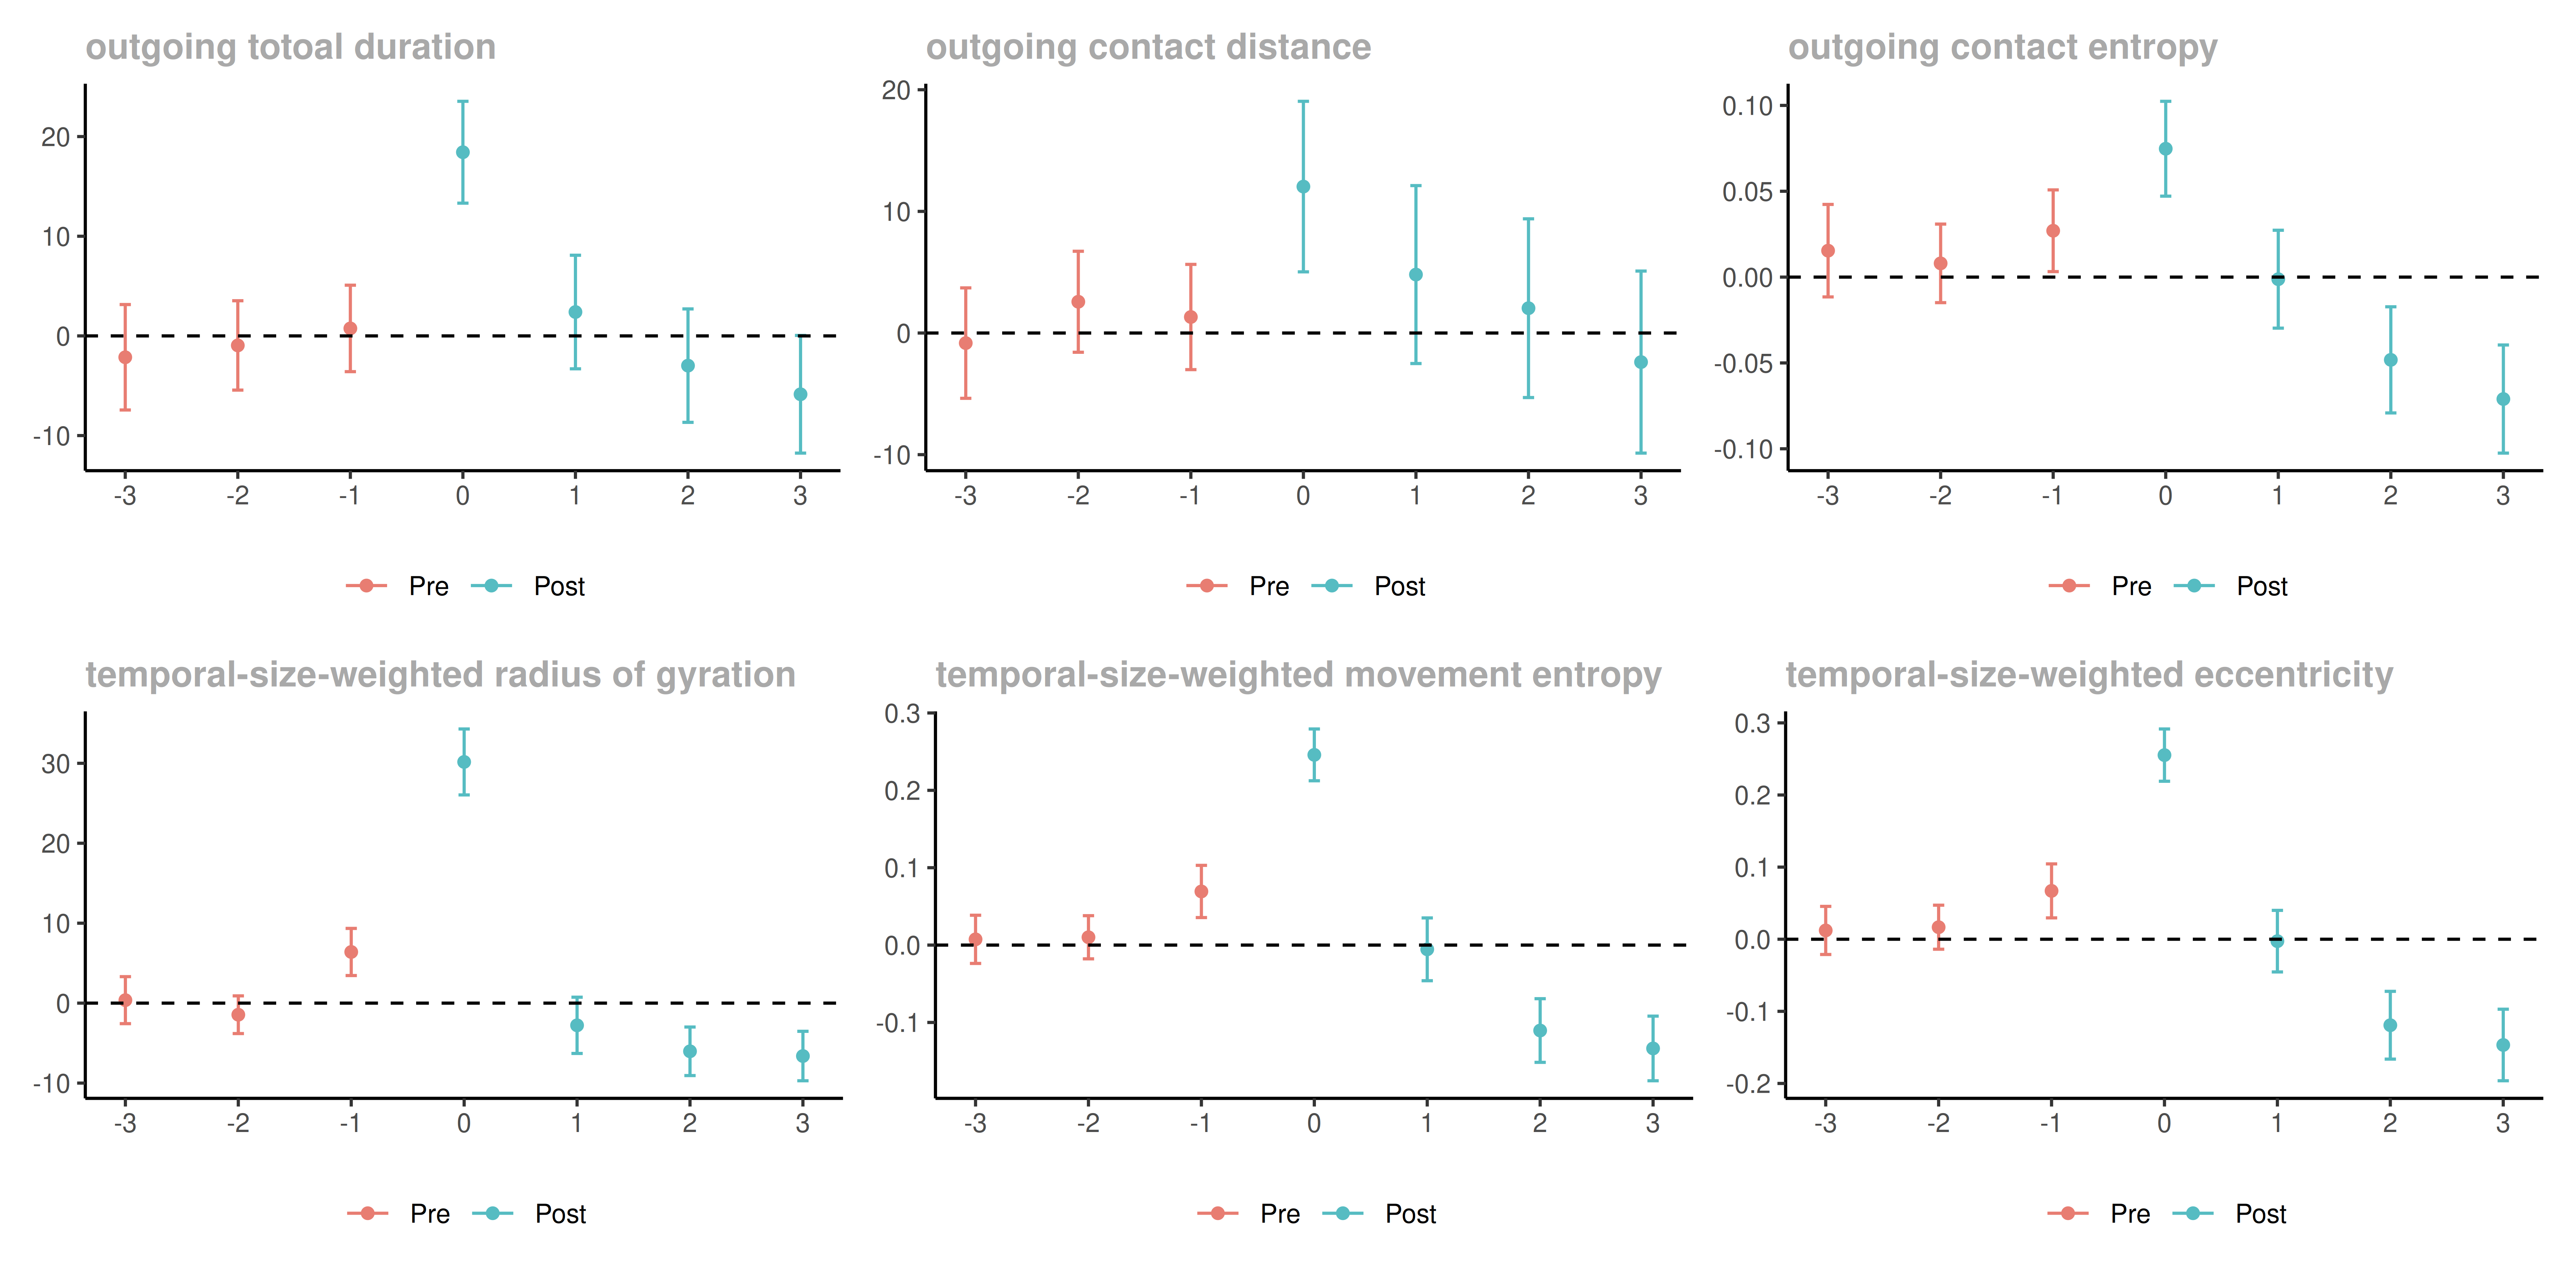
\includegraphics[width=1\textwidth]{figures/csdid/inspect_delta/residential_shift.png}

% \caption*{Note the x-axis is the month relative to the treatment timing.}
\label{fig:select_delta_residential_shift}
\end{figure}

In Figure~\ref{fig:select_delta_residential_shift}, we plot the warmup estimation results of group-time ATT of residential shift on two groups of features.
We can see that the group-time ATT is very often significantly different from 0 in the one-month prior to the residential shift and the ATT in period \( g-1 \) (event time -1) is in the same direction with the period \( g \) (event time 0).
Note that we employ the 95\% confidence bands.
Therefore, we think that the number of months for anticipation \( \delta \)	 should be set to one when discussing treatment effects of residential shift.
% It is interesting to see that in mobility patterns, the anticipation seems to be involved in all three different features, while in mobile communication network features, the anticipation seems to emerge more often in the incoming direction, which potentially indicates the unique characteristics of long-distance contacts in the mobile communication network. For instance, as relocation information spreads through local neighbor networks, distant friends may respond with increased incoming calls to show support, while local contacts can express concern through direct meetings. On the other hand,

Note that for some outcomes, such as outgoing duration and contact distance, it doesn't make sense to claim the existence of anticipation as ATT in event time -1 (period \( g-1 \)	) denoted as \( ATT(-1) \) is insignificant.
However, it won't affect the estimation of post-treatment effect on these outcomes when requiring the anticipation months to be one, i.e., \( g-2 \) is referenced.
This is because as the ``varying'' \textit{base\_period} let $ATT(-1)$ be obtained by referencing period $g-2$, and as the plot shows, $ATT(-1)$ is insignificant, which means the difference, $\mathbb{E}[Y_{i, g-1} - Y_{i, g-2} \mid G_{i, g} = 1]$ is equivalent to the parallel trend. Therefore, it will be differenced out by $\mathbb{E}[Y_{i, g-1} - Y_{i, g-2} \mid G_{i, \infty} = 1]$.

Nevertheless, the situation is not symmetric for outcomes other than outgoing duration and contact distance when we incorrectly set \( \delta = 0 \) while the true value is \( \delta = 1 \).
This asymmetry arises because \( Y_{i,g-1} \) contains an ATT component, and differencing other periods' outcomes against this contaminated baseline distorts the ATT estimates in those periods.
Specifically, the ATT in other periods will be underestimated when treatment effects across periods have the same sign, but amplified when they have opposite signs.

Regarding the treatment of smartphone adoption, it seems to be unfair to claim the existence of anticipation, and through the plot, we don't find the evidence of pre-treatment shifts in outcomes, therefore we will set $\delta$ to 0.

\begin{figure}[h!]
\centering
\caption{Aggregate Event Study of Smartphone Adoption with No Anticipation}
\vspace{0.1cm}

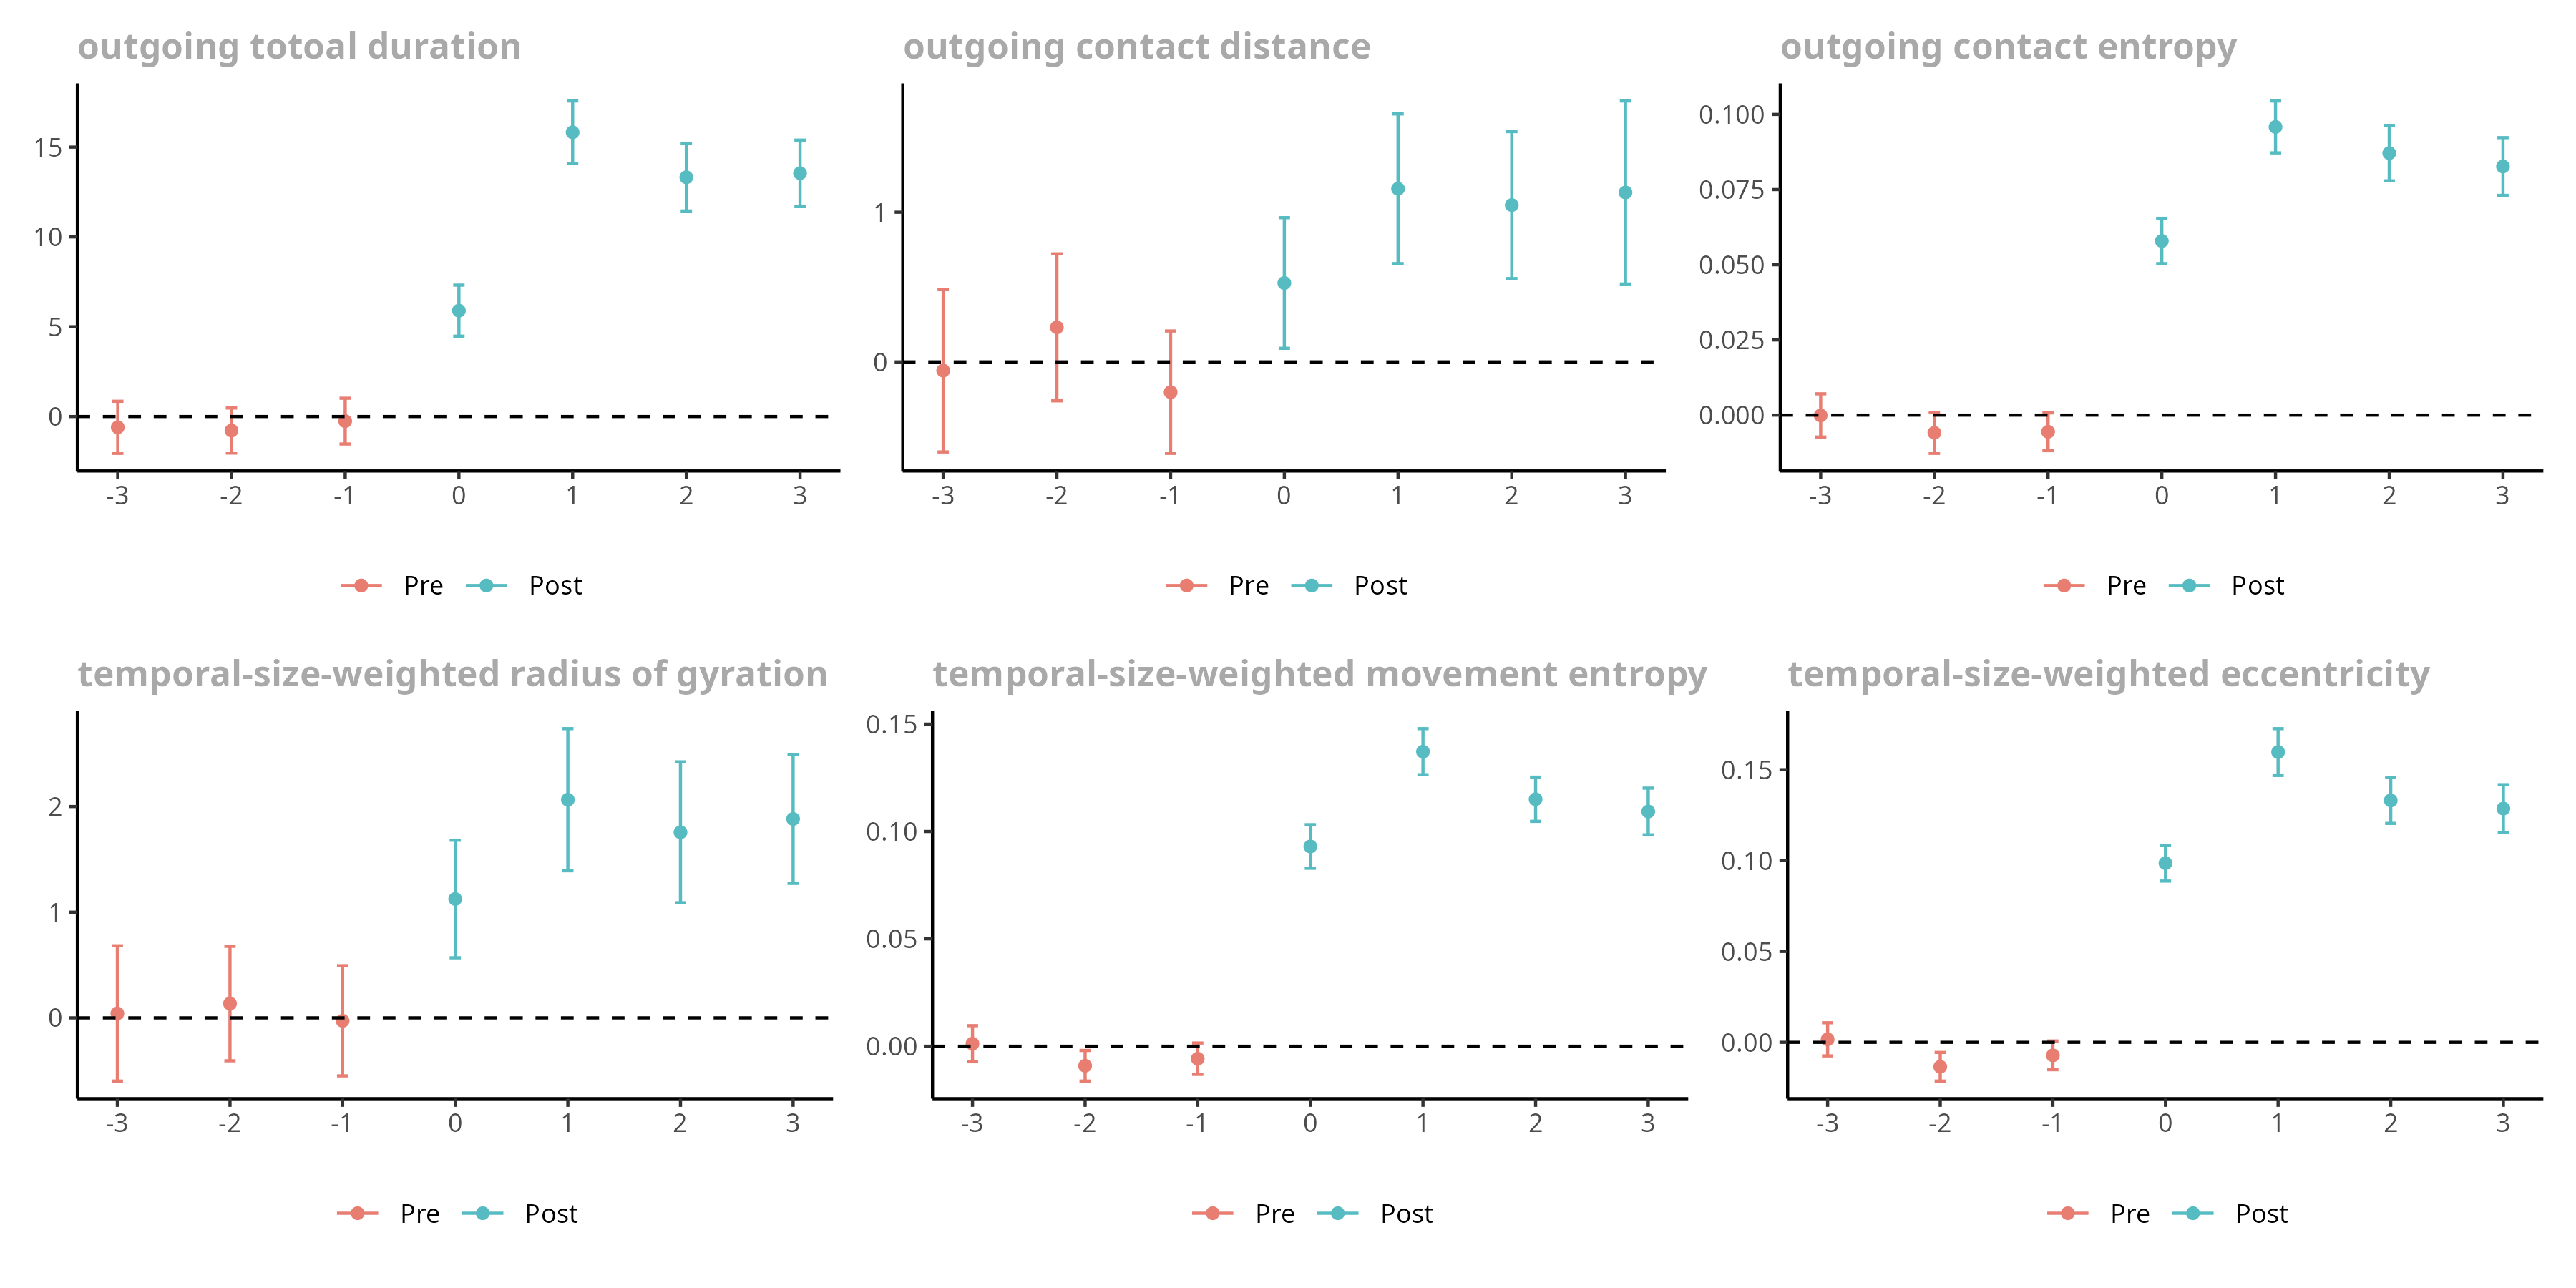
\includegraphics[width=1\textwidth]{figures/csdid/inspect_delta/smartphone_adoption.png}

% \caption*{Notes: }
\label{fig:select_delta_smartphone_adoption}
\end{figure}
